\begin{figure}[!t]
    \centering 
    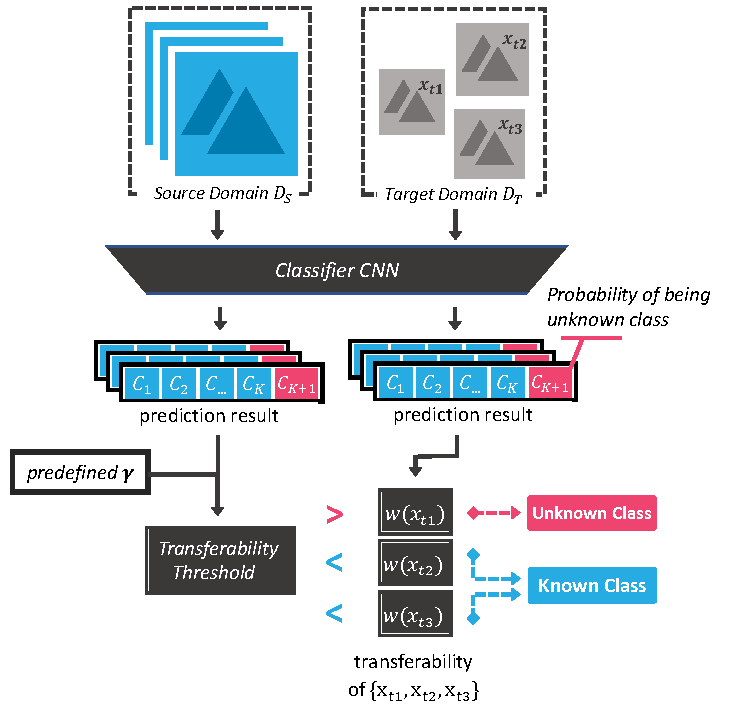
\includegraphics[width=0.48\textwidth]{contents/figures/pdf/selection.pdf} 
    \caption{
        The procedure of transferability based sample selection. 
        Given a batch of training samples, we calculate a transferability threshold by averaging transferability scores of source domain samples, and further tweak it during the training process.
        Then we select target samples whose transferability exceeds threshold as samples from the known classes, \textit{e.g.}, $x_{t2}$ and $x_{t3}$ are select for domain adversarial training. 
    } 
    \label{figure: selection} 
\end{figure}